\begin{tikzpicture}[x=1cm, y=1cm, font=\sffamily\footnotesize,
  ptitle/.style={anchor=west, font=\sffamily\bfseries\small, text=narrareddeep},
  textbox/.style={draw=phaseA!60, fill=phaseA!6, rounded corners=2pt, inner sep=4pt, anchor=north west,
                  align=left, font=\sffamily\scriptsize},
  lbl/.style={draw=#1, fill=white, fill opacity=0.9, text opacity=1, rounded corners=1pt, inner sep=1.6pt,
              line width=0.6pt, font=\sffamily\scriptsize},
  lblkey/.style={draw=#1, fill=white, fill opacity=0.95, text opacity=1, rounded corners=1pt, inner sep=1.8pt,
                 line width=1.0pt, font=\sffamily\scriptsize\bfseries},
  lead/.style={draw=#1, line width=0.7pt},
  path/.style={-{Latex[length=2.6mm, width=2.4mm]}, draw=black!85, line width=1.6pt},
  imgcap/.style={anchor=north, font=\sffamily\scriptsize, text=black!60},
  chip/.style={draw=black!30, fill=white, rounded corners=6pt, inner sep=2.5pt, font=\sffamily\footnotesize},
  flow/.style={-{Latex[length=1.6mm]}, draw=black!50, line width=0.6pt},
  lab/.style={anchor=east, font=\sffamily\footnotesize, text=black!75},
  txt/.style={anchor=west, font=\sffamily\footnotesize, text=black!75}]

\node[ptitle] at (0,0) {(a) One WebShop session in the official web app (evaluation session 0)};
\node[anchor=south west, align=left, text width=5.40cm, font=\sffamily\scriptsize, text=black!75, inner sep=1pt] at (0.000,-1.650) {The start page shows the request and a search box.};
\node[anchor=north west, inner sep=0] at (0.000,-1.750) {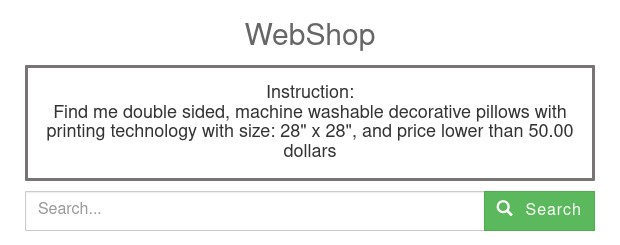
\includegraphics[width=5.500cm]{figures/cases/ws_search.jpg}};
\draw[black!35, line width=0.4pt] (0.000,-1.750) rectangle ++(5.500,-2.173);
\node[anchor=south west, align=left, text width=3.85cm, font=\sffamily\scriptsize, text=black!75, inner sep=1pt] at (5.800,-1.650) {After \texttt{search[double sided machine washable decorative pillows 28 x 28]}: 50 results, 10 per page.};
\node[anchor=north west, inner sep=0] at (5.800,-1.750) {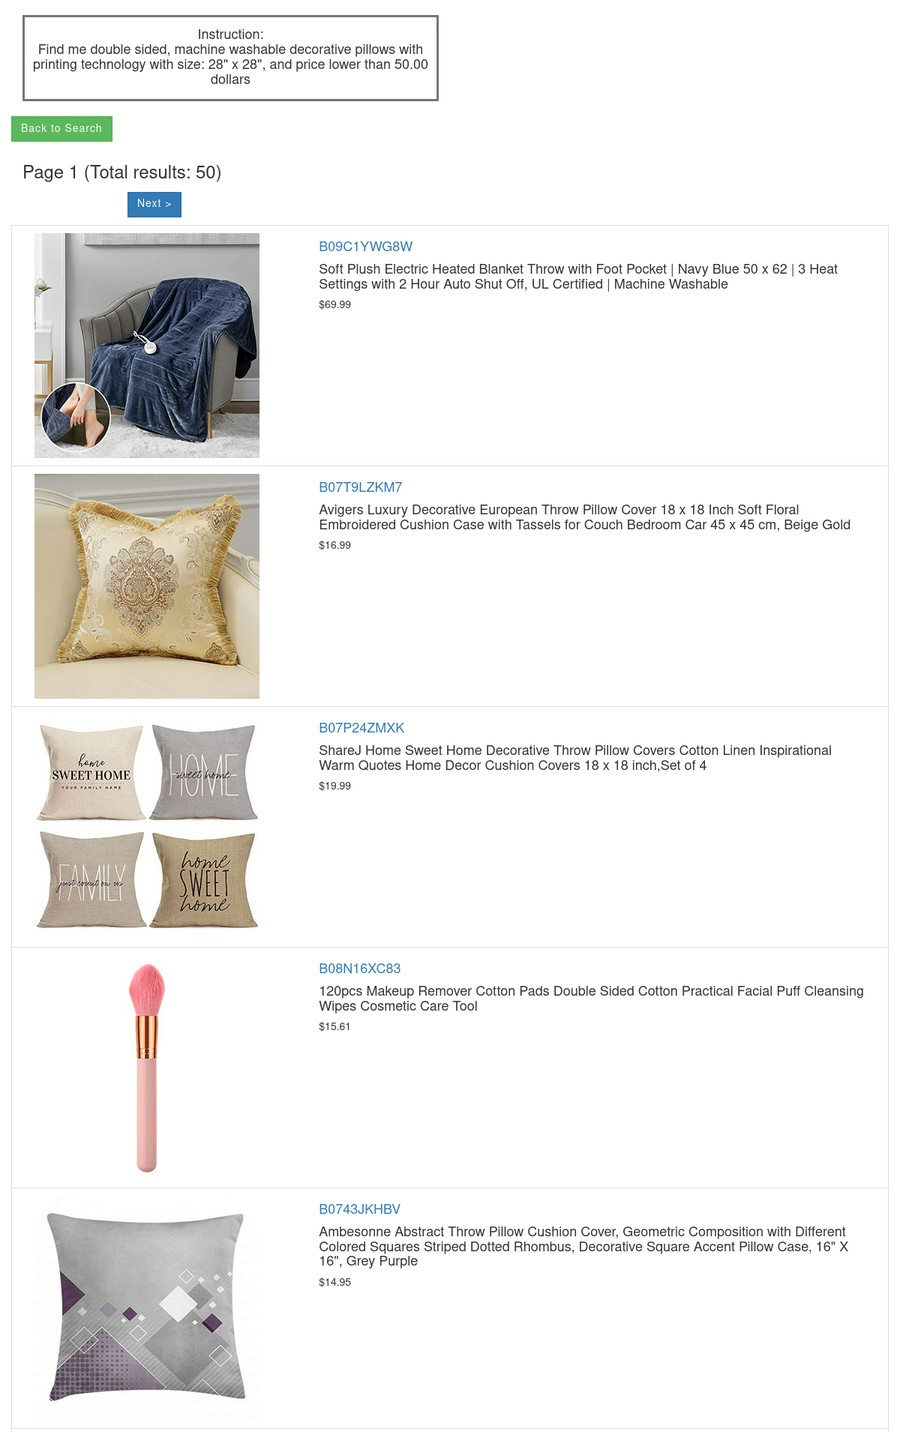
\includegraphics[width=3.950cm]{figures/cases/ws_results.jpg}};
\draw[black!35, line width=0.4pt] (5.800,-1.750) rectangle ++(3.950,-6.285);
\node[anchor=south west, align=left, text width=4.85cm, font=\sffamily\scriptsize, text=black!75, inner sep=1pt] at (10.050,-1.650) {After \texttt{click[B0743JKHBV]}: the product page, with its size options and a \textit{Buy Now} button.};
\node[anchor=north west, inner sep=0] at (10.050,-1.750) {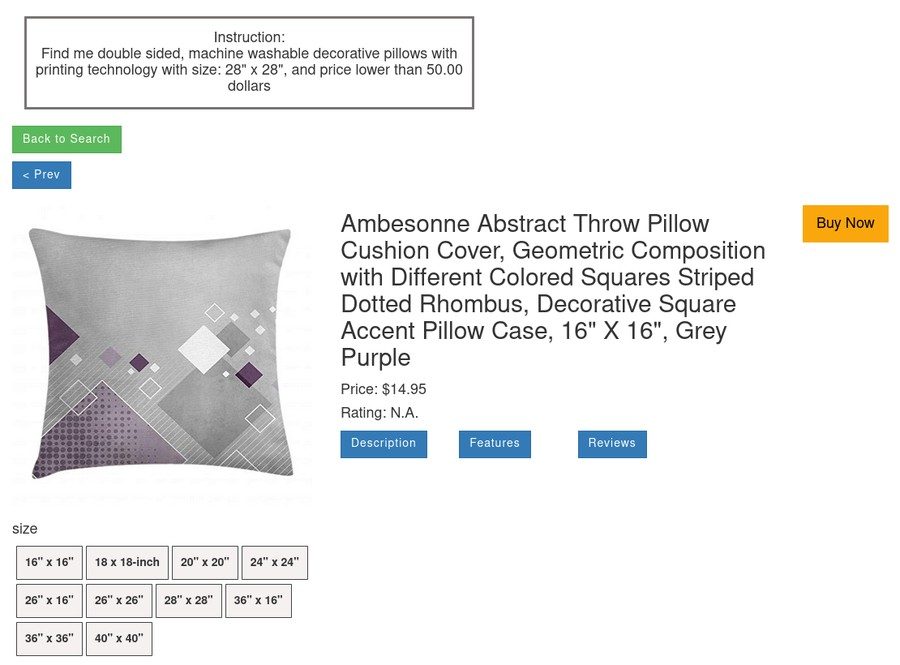
\includegraphics[width=4.950cm]{figures/cases/ws_product.jpg}};
\draw[black!35, line width=0.4pt] (10.050,-1.750) rectangle ++(4.950,-3.658);
\node[anchor=south west, align=left, text width=4.85cm, font=\sffamily\scriptsize, text=black!75, inner sep=1pt] at (10.050,-6.528) {After \texttt{click[28\textquotedbl{} x 28\textquotedbl{}]} and \texttt{click[Buy Now]}: the episode ends; the score box (green) shows reward 1.0.};
\node[anchor=north west, inner sep=0] at (10.050,-6.608) {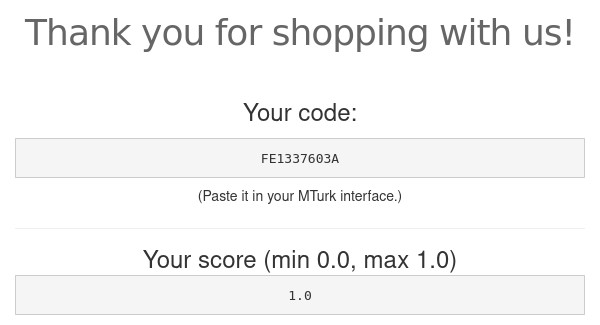
\includegraphics[width=4.950cm]{figures/cases/ws_score.jpg}};
\draw[black!35, line width=0.4pt] (10.050,-6.608) rectangle ++(4.950,-2.681);
\draw[liftpositive, line width=1.2pt, rounded corners=1pt] (5.835,-6.960) rectangle (9.715,-8.026);
\node[lblkey=liftpositive, anchor=center] (hl) at (7.775,-8.355) {the requested product (5th)};
\draw[lead=liftpositive] (hl) -- (7.775,-8.026);
\draw[dimA, line width=1.2pt, rounded corners=1pt] (10.902,-4.957) rectangle (11.277,-5.155);
\node[lblkey=dimA, anchor=west] (hl) at (11.700,-5.056) {\texttt{click[28\textquotedbl{} x 28\textquotedbl{}]}};
\draw[lead=dimA] (hl) -- (11.277,-5.056);
\draw[dimF, line width=1.2pt, rounded corners=1pt] (14.461,-2.872) rectangle (14.940,-3.087);
\node[lblkey=dimF, anchor=east] (hl) at (14.340,-2.674) {\texttt{click[Buy Now]}};
\draw[lead=dimF] (hl) -- (14.461,-2.872);
\draw[liftpositive, line width=1.2pt, rounded corners=1pt] (10.166,-8.868) rectangle (14.885,-9.215);
\node[textbox, text width=5.20cm] at (0.000,-4.223) {\textbf{What the reward checks.} The purchase is compared with the request:\\[1pt]\textbullet\ attributes: double sided, machine washable, printing technology\\\textbullet\ option: size 28\textquotedbl{} x 28\textquotedbl{}\\\textbullet\ price: lower than \$50.00\\\textbullet\ product type: the title must match the request\\[2pt]The reward is the share of matched attributes, options, and price, times the type match; here everything matches, so it is 1.0. A session allows at most 15 actions, and the store holds 1{,}000 products. The ranking shown comes from our BM25 stand-in for the search index.};
\draw[flow, line width=1pt] (5.530,-2.850) -- (5.770,-2.850);
\draw[flow, line width=1pt] (9.780,-2.850) -- (10.020,-2.850);
\draw[flow, line width=1pt] (9.930,-5.108) |- (10.020,-7.108);
\node[ptitle] at (0,-10.039) {(b) What happened: \texttt{Qwen3-8B}, 100 sessions};
\node[lab] at (1.650,-10.639) {no memory};
\fill[phaseA!35, rounded corners=1pt] (1.750,-10.489) rectangle ++(4.666,-0.3);
\node[txt] at (6.496,-10.639) {mean reward 0.194};
\node[lab] at (1.650,-11.099) {memory};
\fill[salmon!60, rounded corners=1pt] (1.750,-10.949) rectangle ++(2.508,-0.3);
\node[txt] at (4.338,-11.099) {mean reward 0.105};
\node[txt] at (9.600,-10.639) {paired change per session:};
\fill[salmon!60] (9.600,-10.939) rectangle ++(1.080,-0.36);
\node[font=\sffamily\footnotesize] at (10.140,-11.119) {20};
\node[font=\sffamily\scriptsize, text=black!65, anchor=north] at (10.140,-11.339) {declined};
\fill[black!12] (10.680,-10.939) rectangle ++(3.888,-0.36);
\node[font=\sffamily\footnotesize] at (12.624,-11.119) {72};
\node[font=\sffamily\scriptsize, text=black!65, anchor=north] at (12.624,-11.339) {unchanged};
\fill[qwenmint!55] (14.568,-10.939) rectangle ++(0.432,-0.36);
\node[font=\sffamily\footnotesize] at (14.784,-11.119) {8};
\node[font=\sffamily\scriptsize, text=black!65, anchor=north] at (14.784,-11.339) {improved};
\end{tikzpicture}
